%! Author = jacobcarlson
%! Date = 4/26/23

\section{Opcode Set Collection}

The executables in the training set are all from machines running the Windows operating system,
primarily Windows 7\cite{lester}, but their opcode sets vary and a total of 1,457 different opcodes
were found in the training set.
Only $1.9\%$ of those opcodes occur in more than $25\%$ of the training samples, this means that most of the opcodes
will not make a difference when being used to make comparisons between files.
When an opcode does not occur, the distribution would just be uniform since there were no occurrences to
derive jumps from.
Comparing uniform distributions to ground truth distributions will not provide any meaningful information, so an effort
was made to find an optimal and commonly occurring set of opcodes.

\subsection{Benign, Malicious}

Simple opcode sets were derived by taking the $50$ most occurring opcodes from different sample sets of benign and
malicious files only.
This ensured that when creating distributions for individual executables, there was a good chance that most
of the opcodes had enough occurrences to yield a meaningful distribution.
$86\%$ of the opcodes overlapped between the two sets, so the distribution sets share most of the same data.
This reduces the chances of an opcode from one set being infrequent when compared against either opcode set.
The heatmaps in Figure \ref{fig:example_heatmaps}, display a consistent pattern of similarity between
ground truth samples of the same class over both classes in each opcode set heatmap.
The heatmaps look similar due to the number of overlapping opcodes in each set.

Table \ref{tab:benignMalicious} shows the average accuracies and standard deviations of the benign and malicious opcode
set when tested over 40 different combinations of ground truth and training samples.

\begin{table}[H]
    \begin{center}
        \captionsetup{justification=centering}
        \caption{Average Accuracy of Benign and Malicious Opcode Sets}
%        \footnotesize{Average test accuracies and standard deviations are obtained using ten different sample ground
%        truth sample pairs, tested 4 times each using a different random seed each time to differ the data. Resulting
%        in 40 different test cases.}
%        \footnotesize{$Bins: 100,\; KL\; Divergence\; Method: KL(X||dist),\; Model: MLP Scaled$\\}
        \begin{tabular}{c|c}
            \textbf{Benign} & \textbf{Malicious}\\
            \hline
            $88.1\% \pm 1.1\%$ & $88.7\% \pm 1.7\%$ \\
        \end{tabular}
        \label{tab:benignMalicious}
    \end{center}
\end{table}

The accuracies of each opcode set are not significantly different in terms of their average and standard deviations
(Figure \ref{tab:benignMalicious}); however, the malicious set was shown to be the more accurate set
$(Z=3.34, p=1.00)$, using a Wilcoxon Signed Rank test  where the input data is the difference between the
accuracies under the same conditions - $(KL\; Divergence\; Method:\; KL(X||dist))$,



\subsection{Union, Intersction, Disjoint}
Without using more in-depth approaches, the union, intersection, and disjoint of the benign and malicious opcode sets
were tested as opcode sets.
The union and intersection of the benign and malicious opcode sets only differ slightly from the original
sets, since those sets were so similar.
The benign and malicious sets each have seven opcodes that do not belong to the other set, so the benign and
malicious union set has $57$ opcodes while the intersection set has $43$ opcodes.
These sets both provide a valuable insight since the union set has more opcodes, which are frequent to at least one set,
while the intersection set has fewer opcodes, but they are all frequent to both opcode sets.

\begin{center}
    Benign - Intersection:\\
    $[abcb,\; cmpw,\; jns,\; lock,\; movzwl,\; sbbb,\; sete]$\\
    Malicious - Intersection:\\
    $[call,\; jmpl,\; leave,\; popl,\; retl,\; sarl,\; shll]$
\end{center}

When using the previously constructed sets the goal was to find opcodes that occurred frequently enough to create
a strong distribution, but the idea behind the disjoint set was to potentially use the lack of distribution to
illustrate difference, as was found in Bilar\cite{bilar}.
Opcodes that are common to malicious files but not benign files, and vice versa, were combined in the disjoint set.
Figure \ref{fig:unionIntersectionDisjoint}, introduces the heatmaps that show the summed KL Divergence values over all
opcodes in the union, intersection, and disjoint opcode sets.

\begin{figure}[H]
    \centering
    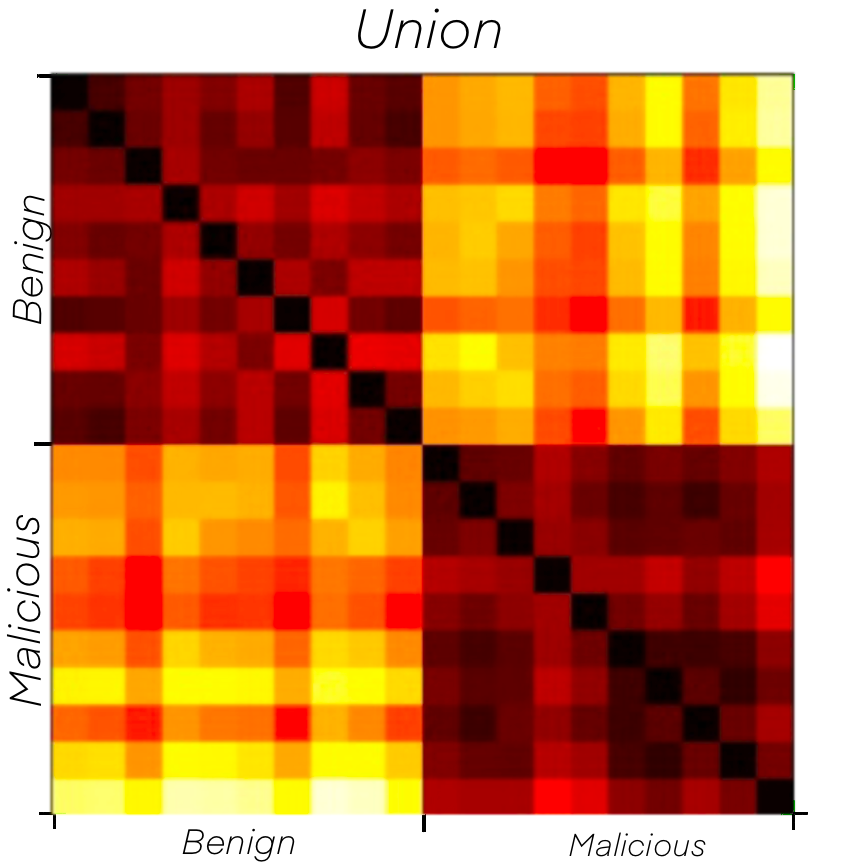
\includegraphics[width=0.2\textwidth]{jump_union}\hspace{1em}%
    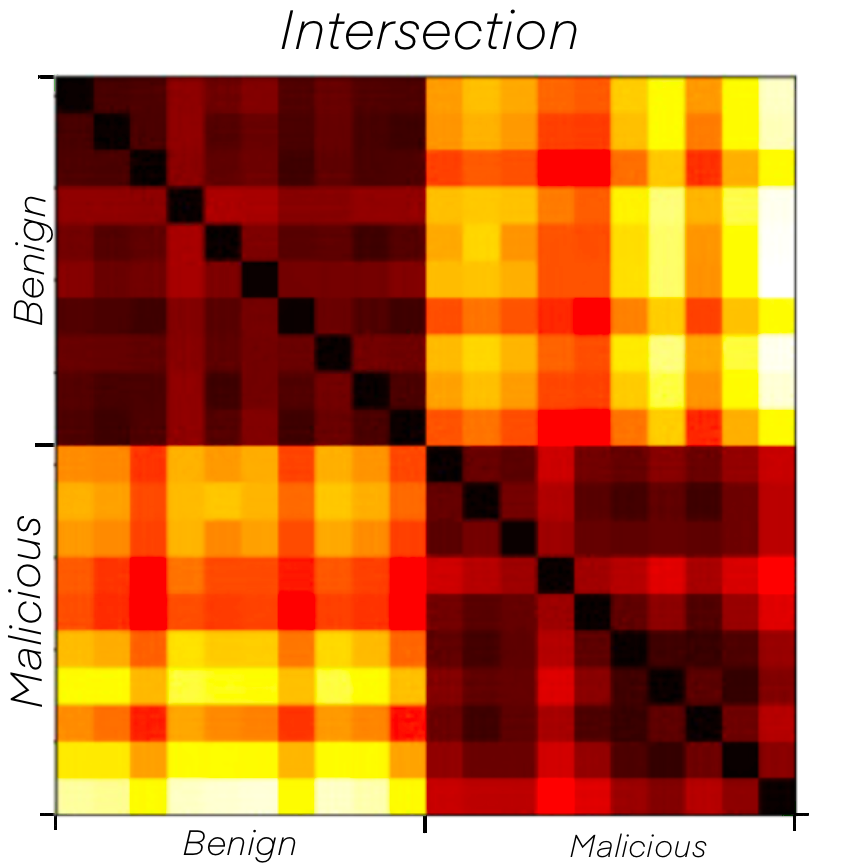
\includegraphics[width=0.2\textwidth]{jump_intersection}
    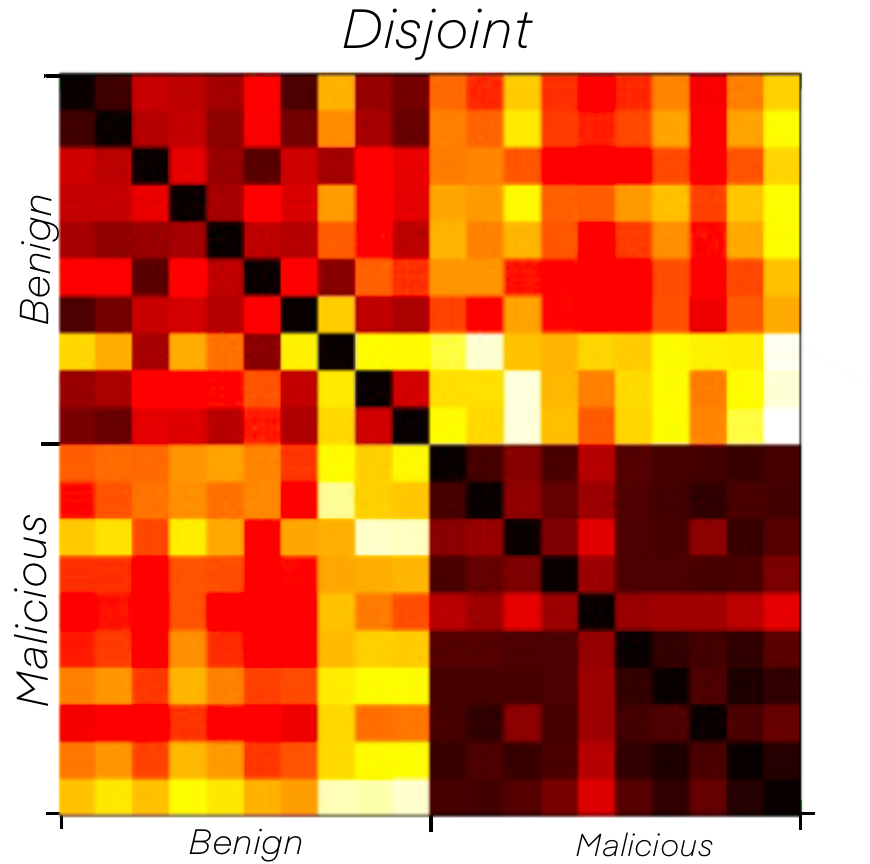
\includegraphics[width=0.2\textwidth]{jump_disjoint}
    \centering
    \caption{
        Union, Intersection, Disjoint Heatmaps
    }
%    \footnotesize{Heatmaps for 20 ground truth samples, 10 of each class. Cells of a darker color indicated lower
%    Kullback-Leibler Divergence values, while cells of a lighter color indicate higher KL Divergence values.}
    \label{fig:unionIntersectionDisjoint}
\end{figure}

The union and intersection opcode set heatmaps (Figure \ref{fig:unionIntersectionDisjoint}) each show a strong
degree of class similarity and intra-class dissimilarity.
This makes sense since both the malicious and benign classes heavily overlapped and also showed the same
characteristics.
This potential for increasingly different KL Divergence values when using infrequent opcodes is illustrated in
the disjoint heatmap (Figure \ref{fig:unionIntersectionDisjoint}), which does not follow as clear of a pattern
as the previous sets heatmaps.
There is a lower more consistent summed KL divergence between the malicious ground truth samples, while the Benign
samples seems to be much more erratic.

Table \ref{tab:unionInterectionDisjoint} shows the accuracies and standard deviations of the union, intersection,
and disjoint opcode sets when tested over 40 different combinations of ground truth and training samples.
Table \ref{tab:uidvsMalicious} compares the union, intersection, and disjoint opcode sets to malicious opcode set
under the same conditions, displaying the probability of the given opcode set being more accurate than the malicious
opcode set tested using the Wilcoxon Signed Rank Test.

%No opcode set was consistently more accurate than the malicious opcode set.

\begin{table}[H]
    \begin{center}
        \captionsetup{justification=centering}
        \caption{Average Accuracy of Union, Intersection, Disjoint Opcode Sets}
%        \footnotesize{Average test accuracies and standard deviations are obtained using ten different sample ground
%        truth sample pairs, tested 4 times each using a different random seed each time to differ the data. Resulting
%        in 40 different test cases.}
        \begin{tabular}{c|c|c}
            \textbf{Union} & \textbf{Intersection} & \textbf{Disjoint}\\
            \hline
            $88.6\% \pm 1.6\%$ & $88.0\% \pm 1.3\%$ & $84.9\% \pm 1.6\%$ \\
        \end{tabular}
        \label{tab:unionInterectionDisjoint}
%        \footnotesize{\\$KL\; Divergence\; Method: KL(X||dist)$}

    \end{center}
\end{table}

\begin{table}[H]
    \begin{center}
        \captionsetup{justification=centering}
        \caption{Probability of Opcode set yielding higher accuracy than Malicious Opcode Set}
%        \footnotesize{Z scores and Probabilities of opcode sets being more accurate than the malicious opcode set when
%        tested with a Wilcoxon Signed Rank test, using the differences between the accuracies of samples tested on the
%        same data under the same conditions.}
%        \footnotesize{\\$KL\; Divergence\; Method: KL(X||dist)$}
        \begin{tabular}{l|S|S}
            \textbf{Opcode Set} & \textbf{Z} & \textbf{p}\\
            \hline
            Union & -0.35 & 0.366\\
            Intersection & -3.28 & 0.000\\
            Disjoint & -5.28 & 0.000\\
        \end{tabular}
        \label{tab:uidvsMalicious}
    \end{center}
\end{table}

Out of the newly tested opcode sets, the union of the benign and malicious opcodes was the most accurate, but it still
failed to achieve a higher accuracy than the malicious opcode set.
The malicious opcode set is a subset of the union opcode set, meaning that the seven opcodes that are a part of
the benign set and not the malicious set do not provide any meaningful information and even decrease the accuracy when
compared to the malicious only opcode set.

While the intersection opcode set does not have the benign opcodes that seemingly decreased the accuracy of the
union set, it has a lower accuracy than both the malicious and union opcode sets.
Even though the differences in accuracy are minimal, the opcodes that belong to the malicious opcode
set seem to provide enough meaningful information to significantly boost accuracy.

The disjoint opcode set is much smaller than any of the other opcode sets that have been tested.
Disjoint had an interesting heatmap, showing strong similarity in the malicious opcode set, but had the lowest
accuracy by far.

The malicious opcode set group is the most accurate of the opcode set groups tested.
The malicious set being more accurate than the union opcode set, deters any further tests into opcode set size since
increasing the set size by $14\%$ failed to increase accuracy and any further size increases
will come with increased chance of infrequent opcodes.
The significantly worse accuracy, under $a=0.05$, of the intersection and disjoint sets also leads to the conclusion that
no further steps need to be taken to investigate opcodes that occur frequently in both sets (intersection) or
opcodes that only occur strongly in one set (disjoint).

